\documentclass[twocolumn]{aastex62}
\usepackage{graphicx}
\usepackage{multirow}
\usepackage{enumitem} % for no indent in itemize 
\usepackage[]{algorithm2e}
\newcommand{\vdag}{(v)^\dagger}
\newcommand\aastex{AAS\TeX}
\newcommand\latex{La\TeX}
%\newcommand{\mathcolorbox}[2]{\colorbox{#1}{$\displaystyle #2$}}
%\newcommand{\hlfancy}[2]{\sethlcolor{#1}\hl{#2}}

\received{XXX}
\revised{\today}
\accepted{XXX}

\submitjournal{A\&A}

\begin{document}

\title{Do you trust your reference?}
%On-sky correction of static and quasi-static non-common path aberration with the pyramid wavefront sensor in Extreme Adaptive Optics.
%Dr WHO 1.0: Non-common path aberrations with the pyramid wavefront sensor: how much do you actually trust your reference?
\correspondingauthor{Nour Skaf}
\email{nour.skaf@obspm.fr}

 \author{Nour Skaf} 
 	\affil{LESIA, Observatoire de Paris, Université PSL, CNRS, Sorbonne Universit\'e, Universit\'e de Paris, 5 place Jules Janssen, 92195 Meudon, France}
 	\affil{Subaru Telescope, National Astronomical Observatory of Japan, 650 North A'Ohoku Place, Hilo, HI 96720, USA}
	 \affil{Department of Physics and Astronomy, University College London, London, United Kingdom}


 \author{Olivier Guyon} 
    \affil{Subaru Telescope, National Astronomical Observatory of Japan, 650 North A'Ohoku Place, Hilo, HI 96720, USA}
 	\affil{Steward Observatory, University of Arizona, Tucson, AZ 85721, USA}
 	\affil{Astrobiology Center of NINS, 2-21-1 Osawa, Mitaka, Tokyo 181-8588, Japan}

 \author{Rico Gendrinou} 
 	\affil{LESIA, Observatoire de Paris, Université PSL, CNRS, Sorbonne Universit\'e, Universit\'e de Paris, 5 place Jules Janssen, 92195 Meudon, France}
 	
 \author{Barnaby Norris} 
 	\affil{Sydney Institute for Astronomy, School of Physics, University of Sydney, NSW 2006}

 \author{Vincent Deo}  	
 \affil{Subaru Telescope, National Astronomical Observatory of Japan, 650 North A'Ohoku Place, Hilo, HI 96720, USA}



 	\author{Anthony Boccaletti} 
 	\affil{LESIA, Observatoire de Paris, Université PSL, CNRS, Sorbonne Universit\'e, Universit\'e de Paris, 5 place Jules Janssen, 92195 Meudon, France}
 
 \author{Arielle Betrou-Cantou} 
 	\affil{LESIA, Observatoire de Paris, Université PSL, CNRS, Sorbonne Universit\'e, Universit\'e de Paris, 5 place Jules Janssen, 92195 Meudon, France}

 \author{Jesse Cranney} 
	 \affil{Research School of Astronomy and Astrophysics, Australian National University, Canberra,ACT 2611, Australia}
	 
	 %\author{Céline d'Orgeville} 
	 %\affil{Research School of Astronomy and Astrophysics, Australian National University, Canberra,ACT 2611, Australia}

	  	 \author{Florian Ferreira} 
 	\affil{LESIA, Observatoire de Paris, Université PSL, CNRS, Sorbonne Universit\'e, Universit\'e de Paris, 5 place Jules Janssen, 92195 Meudon, France}

 \author{Damien Gratadour} 
 	\affil{LESIA, Observatoire de Paris, Université PSL, CNRS, Sorbonne Universit\'e, Universit\'e de Paris, 5 place Jules Janssen, 92195 Meudon, France}
	 \affil{Research School of Astronomy and Astrophysics, Australian National University, Canberra,ACT 2611, Australia}	 

\author{Julien Lozi}
	\affil{Subaru Telescope, National Astronomical Observatory of Japan, 650 North A'Ohoku Place, Hilo, HI 96720, USA}
	
\author{Arnaud Sevin} 
 	\affil{LESIA, Observatoire de Paris, Université PSL, CNRS, Sorbonne Universit\'e, Universit\'e de Paris, 5 place Jules Janssen, 92195 Meudon, France}
 	
 \author{Fabrice Vidal} 
 	\affil{LESIA, Observatoire de Paris, Université PSL, CNRS, Sorbonne Universit\'e, Universit\'e de Paris, 5 place Jules Janssen, 92195 Meudon, France}
	 
 \author{Sebastien Vievard}  	
    \affil{Subaru Telescope, National Astronomical Observatory of Japan, 650 North A'Ohoku Place, Hilo, HI 96720, USA}	 
  	\affil{Astrobiology Center of NINS, 2-21-1 Osawa, Mitaka, Tokyo 181-8588, Japan}
	\affil{LESIA, Observatoire de Paris, Université PSL, CNRS, Sorbonne Universit\'e, Universit\'e de Paris, 5 place Jules Janssen, 92195 Meudon, France}
	
	
%\author{Nicolas Doucet} 
%	 \affil{ANU - Canberra Australia}
% \author{Vikram} 
%	 \affil{Leiden}
 %\author{Ben Mazin} 
 %	 \affil{UCSB}

\begin{abstract}

%below is the first astract draft 

%Exoplanetary science is a rapidly growing field in astronomy. However, detecting an exoplanet is very challenging. Over the last couple of decades, ground-based and space-based telescopes became more and more focused on this purpose, using a variety of detection techniques, with the goal to eventually find a nearby planet in the habitable zone with the next generation of instruments. The technique of direct imaging will play a key role in this search. Our project will directly address this challenge of direct detection and characterisation of exoplanets, by developing and testing high precision adaptive optics control techniques to compensate for atmospheric optical turbulence, and the non-common paths aberrations (NCPA). The problem of NCPA is key in direct imaging, as it is one of the main sources of residual speckles in the PSF. The  pyramid  wavefront  sensor  (PWFS),  more  and  more  favored  in  adaptive optics systems for its high sensitivity, is intimately linked with the NCPA correction.  However, the PWFS is non-linear, making its use more challenging.  We will leverage newly available real-time computing capabilities and machine learning numerical tools in order to tackle those problems of NCPA corrections with a PWFS, for boosting image contrast and quality to reveal planet images and better characterise them. We will present the Dr WHO algorithm, which is kind of reinforcement learning approach for frequency lucky imaging and update on-sky the PWFS reference.\\



% below is the submitted for WFS in the VLT era. \\
Exoplanetary science is a rapidly growing field in astronomy. However, detecting directly an exoplanet is very challenging. Over the last couple of decades, ground-based and space-based telescopes became more and more focused on this purpose, using a variety of wavefront control techniques. Our project directly addresses this challenge, by developing and testing high precision adaptive optics control techniques to compensate for atmospheric optical turbulence, the non-common paths aberrations (NCPA). The problem of NCPA is key in direct imaging, as it is one of the main sources of residual speckles in the PSF.
We will present the Dr WHO - Direct Reinforcement Wavefront Heuristic Optimisation - algorithm, a new technique aimed at real-time compensation of NCPA, for boosting image contrast and quality to reveal planet images and better characterize them. It is a kind of reinforcement learning approach for frequency lucky imaging and update on-sky the PWFS reference.
We show that DrWHO does not require accurate wavefront sensor calibration, and is applicable to non-linear wavefront sensing situations. We demonstrate its performance in simulation and on-sky using with the pyramid wavefront sensor (PWFS) sensor.

\end{abstract}

\keywords{Astronomy instrumentation, Adaptive Optics, Extreme Adaptive Optics}


\section{Introduction} \label{sec:intro}

Over the last 30 years, adaptive optics instruments have seen a tremendous progress in terms of development and scientific use, from the first experiments in astronomy with COME-ON, back in 1989, to the most current advanced systems known as extreme AO systems. Many scientific breakthrough came from AO instruments, including the first detection of a planetary companion with VLT/NaCo in 2004 \citep{chauvin2004}, and the first system with four giant planets, HR8799, discovered in 2008 \citep{Marois2008}. In the following years, a second generation of extreme AO (xAO) systems were developed, allowing to go much further in performance in terms of Strehl ratio, contrast, and sensitivity. \cite{Milli2016} made a comparison between AO and xAO systems, in the context of high contrast imaging of exoplanets. In fact, with this scientific goal, there was the need of high contrast requirements on AO systems, so that the wavefront could be corrected to an extreme level. The main current xAO instruments are the GPI, on Gemini South \citep{GPIMacintosh2014,GPIMacintosh2018}; SPHERE on the VLT \citep{BeuzitSPHERE2008}; MagAOx on the Magellan Clay \citep{Males2018MagAOx}; and last but definitely not least, SCExAO on the Subaru Telescope \citep{GuyonSCExAO2010}. 
Those instruments are provided with high rejection coronagraphs, allowing to perform differential imaging and allowing to maintain a slow temporal evolution of aberrations. The main trade-off of those instruments is between angular resolution, AO performance and planet sensitivity \citep{Milli2016}.
Those first generation of xAO systems on 8-10-meter class telescopes will be very valuable in benefiting the generation of xAO instruments on extremely large telescopes.\\

Wavefront sensing is a key feature of any AO system as that measures in real time the distortion of the wavefront. Wavefront sensors need to have enough spatial resolution, and be fast enough to be able to compensate in real-time the atmospheric turbulence, without amplifying and propagating the measurement of the noise. The photon noise is the fundamental limit. The sensitivity is another key driver, as it needs to be able to measure with high accuracy the low orders or aberrations. \cite{Rousset1999} made an overview of wavefront sensing and presented some WFS. 
Back in 1996, \cite{Ragazzoni1996} introduced the PWFS, which has the precious characteristic of being particularly sensitive, way more than any other WFS to date. 
It took nearly a decade before it was used in astronomy, with its first implementation in a very large telescope, the Large Binocular Telescope (2x8.4m) in 2010 by \cite{Esposito2010LBT}. 
However, this PWFS is far from being mastered and fully understood, and still remains an active field of research \citep{Deo2019gain, Chambouleyron2020}.



The AO loop corrects what is given to the WFS. However, the optics after the dichroic, or beamsplitter (cf Figure \ref{fig:NCPA}) induce optical aberrations that aren't seen by the WFS, but impact the science camera. The path after the dichroic is called the "non-common path", and that is where the "non-common path aberrations", or NCPA, come from. 
The phase of NCPA can be defined as follow: 
\begin{equation}
    \Phi_{NCPA} = \Phi_{Residual} - \Phi_{PSF}
\end{equation}

NCPA are a critical limitation in high contrast imaging, and in the field of adaptive optics. Several solutions have been suggested, it yet remains an active field \citep{Vigan2018NCPA, BosFF2020}. In fact, they have a major role in the error budget of the AO system.

They are partially static, and partially quasi-static in time. They can vary with temperature, mechanical deformation on the long term, or with the position of the optics, making them particularly challenging to calibrate. They are typically of the order of tens of nanometers, enough to lead to static and quasi static speckles in the coronagraphic images.

\begin{figure}[h!]
  \centering
    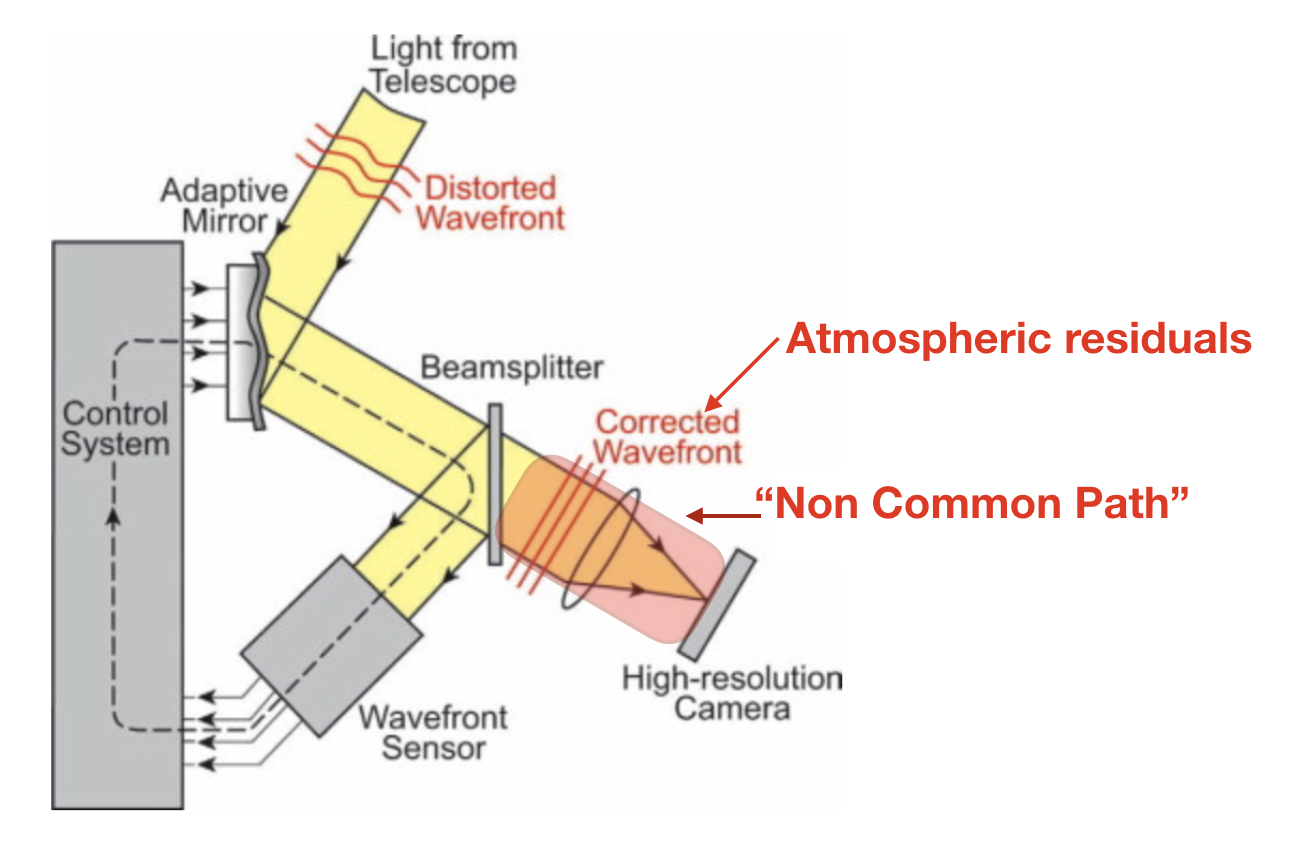
\includegraphics[width=0.5\textwidth]{fig/NCPA.png}
      \caption{AO architecture, with the non-common path highlighted.}
    \label{fig:NCPA}
\end{figure}


\cite{Esposito2015} have been pioneering the way to deal with NCPA with non-linear wavefront sensors, mainly PWFS. 
In fact, as they explain, NCPA are usually corrected by introducing an offset in the WFS signals corresponding to the aberration to correct. However, this is assuming the PWFS is linear, and the calibration with the DM is performed with a previously calculated control matrix, which is true within some extend but mainly wrong, as described earlier. 
As a result, the problems of NCPA and non-linearity of a PWFS are intrinsically linked. They mainly solve the problem by adapting the optical gain with a tracking loop, thanks to a sinusoidal signal added on the DM, in order to have a modulation and a demodulation allowing to derive the value of the optical gain. \textit{to be confirmed, not sure to have understood well.}\\


We will present the Dr WHO algorithm and its results in simulations with the Compass software \citep{Compass}, on the SCExAO bench, and on-sky.\\


\section{Problem statement}
The NCPA is a central issue in direct imaging of exoplanets as it is the main limiting source of error in the PSF. Furthermore, in a system with a PWFS, this problem is intrinsically linked with it. The key issue is to understand what is the \textit{true} reference of the PWFS, that we will call the \textbf{Ideal reference}. In other word, we need to understand what gives a flat wavefront, corrected from all static and quasi-static aberrations and mainly the NCPA. 
The way the reference of the PWFS is currently set, is with an internal light source inside the instrument, before the observations. However, in reality, the \textit{ideal} PWFS reference is constantly evolving\footnote{because of the quasi-static aberrations and the chromaticity of the wavefront}, and is different on sky than with the internal light source. Therefore, a continuous way to measure the \textit{ideal} reference is essential. \\
I would like to emphasise that the \textit{actual} WFS reference as set in the WFS is not the \textit{ideal} reference: the goal is to find what is the closest from it and implement it on the WFS.\\ 
One of the problems is that besides the NCPA, the atmospheric wavefront keeps evolving, therefore we also have atmospheric residuals on top of the NCPA seen by the focal plane camera. This makes the understanding of the \textit{ideal} reference more challenging as well as the NCPA retrieval, since we can't differentiate which aberrations in the focal plane are due to the residuals \textcolor{blue}{develop here}. \\
Yet, another key issue is that the PWFS is non-linear: its response is different depending on the amplitude of the incoming wavefront. Thus, even if we understand what the NCPA are and update the reference of the WFS, there will then be a wrong understanding of the NCPA from the DM because of this non-linearity, therefore a wrong command on the DM, therefore a wrong correction of the NCPA. Adding to that that the NCPA are dynamic, the problem reaches another level of complexity. \ref{fig:pyr_ncpa_pb} gives a schematic view of the problem. 

\begin{figure}[h!]
  \centering
    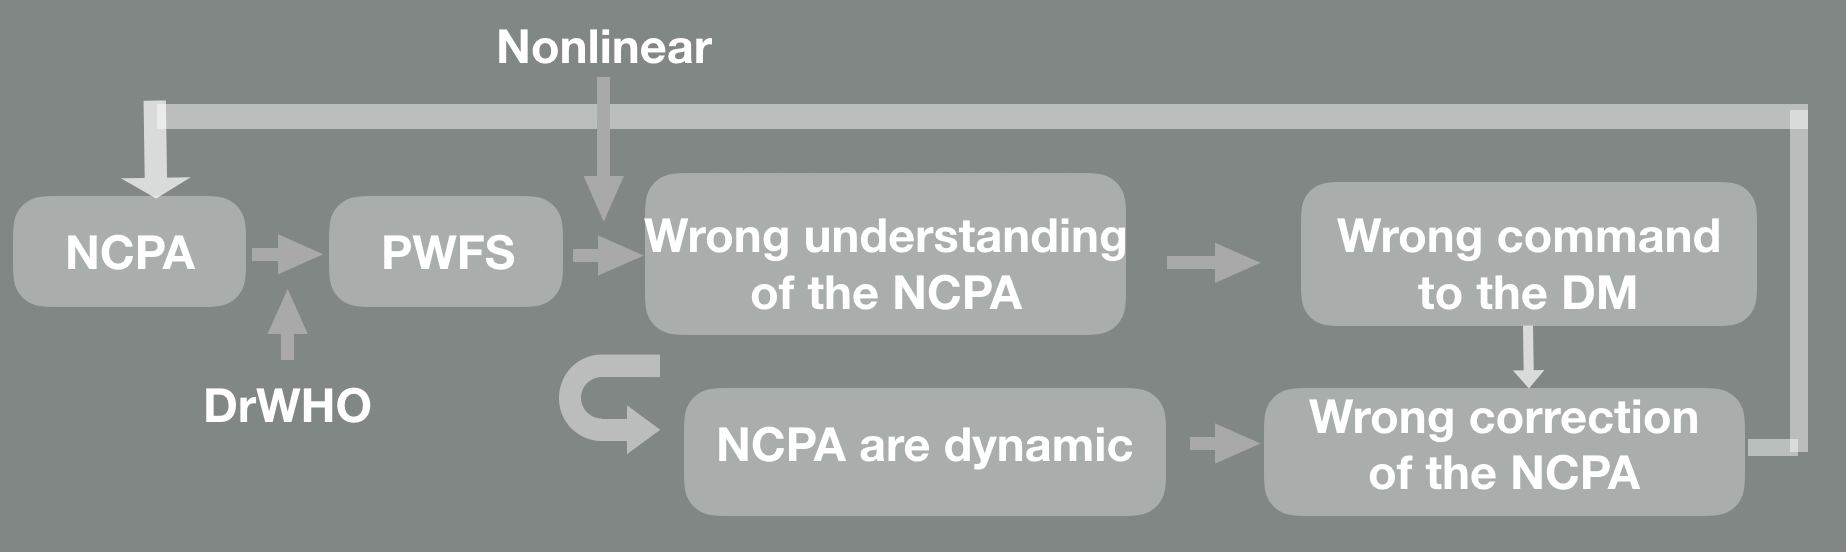
\includegraphics[width=0.45\textwidth]{fig/pyr_ncpa_pb.png}\
      \caption{Schematic description of the NCPA problem linked with the non-linearity of the PWFS.}
    \label{fig:pyr_ncpa_pb}
\end{figure}


\section{Algorithm description}


Since the point is to understand what is the ideal reference of the WFS, we need a continuous way to update the actual reference. DrWHO adopts a kind of reinforcement learning approach to do so, where the "agent" is the PWFS, the action is the actual reference update, with the reward being the Strehl ratio, and the state the NCPA. \\
Here I describe the steps of the algorithms: 
\begin{itemize}
    \item on a 30 seconds timescale, the algorithm identifies the PSF frames with the best 10\% Strehl ratio;
    \item out of those 10\% frames, the corresponding WFS measurements are taken;
    \item those corresponding 10\% WFS measurements are averaged, weighted on the value of the Strehl ratio; 
    \item the resulting WFS frame replaces the WFS reference, with an integrator filter
    \item repeat 
\end{itemize}

Therefore, as the algorithm proceeds, the WFS is continuously rewarded for high quality PSF, and thus the PSF quality improves, and converges towards a better Strehl. \\


\begin{algorithm}[H]
 \KwData{PWFS frames, fast science camera frames.}
 \KwResult{Update the reference of the PWFS}
 initialization: reference of the PWFS with the internal light source\;
 \While{AO loop is running}{
  acquire PWFS and fast science images\;
    \While {Dr WHO loop is running} {
    - take the 10\% best science data\; 
    - take the corresponding WFS images\;
    - average them, weighted on the SR value\;
    - the resulting frame replaces the WFS reference, with a low-pass filter\;
   }{
   keep updating the WFS reference\;
  }
 }
 \caption{Dr WHO algorithm mindset}
\end{algorithm}




\section{Adaptive optics simulations}
Progressing in the algorithm requires numerical simulations; this section presents the AO simulation set up with Compass \citep{Compass}.
Compass is a versatile AO simulator, which has been designed to meet the need of high-performance for the simulation of AO systems, modeling several kinds of AO features, including several kinds of WFS, atmospheric simulations, DMs, telescopes, and RTCs. It offers a suitable environment for simulating single conjugate adaptive optics (SCAO), for very large telescopes (VLT) and extremely large telescopes (ELT) \citep{Vidal2018}.  Simulations of Dr WHO on the Compass software have first been implemented : the main point is to explore the algorithm and implement it first in simulation ahead of implementations on the bench of the SCExAO instrument, with the internal light source, and before the observations. Being able to go back and forth between simulation and instrument have help pin down the issues faced.  \\

\subsection{Simulating SCExAO}
The first step was to simulate SCExAO on Compass, and essentially the pre-correction of the first stage of the AO. In fact, the high contrast instrument on the Subaru Telescope is actually composed of two AO systems, AO188, and then SCExAO. AO188 is the low order AO system, with a curvature wavefront sensor and a DM with 188 actuators on its diameter. SCExAO, however, has a much higher capacity to correct higher orders of aberrations, with a PWFS and a DM of 54 actuators on its diameter. \\

The point isn't necessarily to reproduce exactly SCExAO on Compass, but rather to have a simulation that is close enough to be relevant for testing the algorithm, and predict results on the bench and, later on, on-sky. Table \ref{tab:simuParams} synthetizes the parameters used in the simulation.\\

\begin{itemize}[noitemsep,nolistsep]
    \item $L_0$ = 15m, for simulating the AO188 pre-correction, instead of 100m for uncorrected normal conditions;
    \item The Fried parameter : $r_0$ = 0.16m at 500nm;
    \item The wavelength of the science short exposure camera = 1.65$mu$;
    \item The loop was set to run at 2kHz;
    \item The number of pixels along the diameter of the PWFS = 80;
    \item number of actuators along the diameter of the DM = 54;
    \item The optical throughput coefficient = 50\%;
    \item Only the photon noise is taken into consideration;\\
\end{itemize}



\begin{table}[ht!]
		\centering
		\caption{%
			AO numerical simulations parameters.
		}
		\label{tab:simuParams}
		
		\renewcommand{\arraystretch}{1.2}
		\begin{tabular}{ll}
			\multicolumn{2}{c}{\textbf{Numerical simulation configuration}}\\
			\hline\hline
			\multirow{4}{*}{Telescope} & $D$ = 8.3~m diameter\\
			& Subaru pupil \\
			& $\quad$798 aggregated hexagons\\
			& $\quad$No support spiders\\
			\hline
			\multirow{5}{*}{Turbulence layer} & von Kármán, ground layer only\\
			& $r_0$ = 0.16 at 500~nm \\ % variable in a\\
			%& $\quad$useful range of 7.0 - 35.0~cm\\
			& L$_0$ = 15~m\\
			& $||\overrightarrow{\vect{v}}||$ = 10~m.s$^{-1}$\\
			\hline
			PWFS & \\
			\multirow{2}{*}{$\quad$Subapertures} & 92$\times$92 -- pixel size 42~cm.\\
			& 24,080 useful pixels\\
			$\quad$Wavelength & Monochromatic, 658~nm\\
			$\quad$Throughput & 50\% \\
			$\quad$Modulation & Circular, 4~$\frac{\lambda}{D}$ radius\\
			%$\quad$Readout noise & 0.3~$e^{-}$\\
			\hline
			Focal Plane Camera & \\
			$\quad$Wavelength & Monochromatic, 1.65~$\mu$m\\ 
			\hline 
			Source & On-axis natural guide star\\
			Guide star flux & Zero point: $2.6 \times 10^{10}$~ph.s$^{-1}$.m$^{-2}$\\
			\hline
			\multirow{5}{*}{Adaptive mirrors} & Tip-tilt mirror\\
			& Hexagonal M4 model pattern\\
			& $\quad$Pitch of 54~cm\\
			& $\quad$Coupling of 0.24\\
			& $\quad$4,310 controlled actuators\\
			& Both with infinite bandwidth\\
			\hline
			RTC controller & \\
			$\quad$Loop rate & 2~kHz\\
			$\quad$Method & Linear modal integrator\\
			$\quad$Latency & Data flow 1 frame + MVM 1 frame\\
			$\quad$Basis & DM Karhunen-Loëve basis\tablefootmark{(a)}\\
			\hline
		\end{tabular}
		\tablefoot{
			\tablefoottext{a}{- \cite{Compass}}
		}
	\end{table}


\textcolor{blue}{talk about how the interaction matrix is taken, how we take care of initializing the PWFS reference, how we deal with the noise}
 

\subsection{Dr WHO on Compass}
Dr WHO on Compass was implemented in Python
To make this convergence faster, the DM was poked with random phases with an amplitude comparable to the one of the NCPA, in order to increase the probability of lucky imaging. \\

\textcolor{blue}{describe why you need to reopen - re-zero the loop at each Dr WHO iteration.}\\

\section{Dr WHO on SCExAO}

Dr WHO was then deployed on the SCExAO instrument, which is located on the infrared nasmyth platform of the Subaru Telescope, after the AO188 instrument. 
\textcolor{blue}{add a schema to show how SCExAO and AO188 work, with focal plane camera and PWFS}
The instrument is provided with a PWFS in the 600-950 wavelength range \citep{Lozi2019PWFS}. The real time control (RTC) of the AO system is managed by the CACAO software - Compute And Control for Adaptive Optics - \citep{cacao2018} \textcolor{blue}{describe how cacao relies on HPC and is GPU based}. The diameter of the DM has 45 actuators on the active pupil, giving a control radius of 22.5$\lambda$/D. We use the CACAO software to interact with the system and implement the algorithm, to communicate between the PWFS and the DM. The DM is 12 channels, on which several corrections are implemented from additional wavefront sensors or wavefront control techniques \textcolor{blue}{add citations of examples of WF control techniques that use the DM}. Furthermore, CACAO updates the reference of the PWFS by adding an offset which prevents the AO loop to cancel out the commands of the wavefront control sensing techniques with the DM. 
There are several scientific cameras downstream SCExAO, including CHARIS and REACH in the near-infrared \textcolor{blue}{add citation for both}, VAMPIRES in the visible \citep{vampires2015}. 


\subsection{Data synchronisation}

On SCExAO, the PWFS and the short exposure focal plane camera run at different frequencies, hence the need of synchronising the data streams. 
This can be done directly on the files that are on the hard drive, but not in real time. Indeed, Dr WHO doesn't need to have real time frames, since a loop of the algorithm is several seconds long. 
A script for dealing with is has been implemented. Three inputs are required: the two streams to synchronize - here the PWFS and the focal plane camera -; and the time interval, which is the frequency at which the two streams will be re-sampled. \\
For example, if the focal plane camera runs at 1kHz, the PWFS camera runs at 2kHz, and we want a stream at 3kHz : we want both of those streams synchronized at this frequency difference. Then, the synchronization script will wait for fits cubes and the timing files to appear on the hard drive, read them and re-sample them to the same time baseline. This script is optimized to handle missed frames, and if the timing isn't continuous. Furthermore, it does a linear interpolation of the streams. For example, if we want a 1ms frame, and there is a half PWFS cube and half of the focal plane camera, it will do the weighted average. 
This scripts then provides an other stream of data cubes of the required length (which is set ahead), that are saved on the disk. As said above, it isn't real time as there is a latency to it, however it does spill fits files with the sampling and the timing information. Choosing the length of the data cubes is linked with the latency we need for Dr WHO. This script needs to be launched once only, then it catches up as the AO loop is running. 

\subsection{Details of specific Scexao Dr WHO }

The way it's done is in 4 steps: \\
1- get the 2 data streams; \\
2- take the the timing files; \\ 
3- create the synchronized files and generate a *.sync.fits;\\ 
4- frame selection with Dr WHO (with the script \textit{cacao-selectWFS}. \\

The input parameters to run the whole algo ( \textit{cacao-WFSrefTunePSFloop} ) are as follow, in \textit{runDrWHO} (bash script) : 
\begin{itemize}[noitemsep,nolistsep]
    \item starttime : in Unix time second
    \item data path of the PyWFS and focal plane data, for the synchronization 
    \item the number of iterations you want Dr WHO to run 
    \item the selection fraction
    \item the optimized mode (???)
    \item the Exposure time (OutExpTime)
    \item the time lag between the PSF and WFS streams
    \item the time span of the Dr WHO loop 
\end{itemize}

The algo runs on scexao1, the new references are all saved as imwfsbest.fits and sends it directly to scexao5 (AOloop/DrWHO directory) to apply the new reference on the PyWFS thanks to the bash script \textit{cacao-WFSref}.  


\subsection{PSF selection fraction optimization}
We need Dr WHO to converge the fastest way and therefore to figure out what is the best selection fraction rate of the PSF. We first did some tests on two telemetry blocks, following each other but with the same WFS reference, thus independent. On the first block, we save all the final references given for each iteration of the algorithm for each selection fraction. While on the second block, which is independent, we look at the WFS image that is the closest from the reference given by Dr WHO on the first block. The point is to figure out which selection frame gives the best PSF. 


\section{Results}

\subsection{Simulation}
\subsection{Telemetry}
The first step taken was to look at the telemetry of previous nights and on one iteration of the Dr WHO loop, do some kind of reverse engineering to figure out the success level of the iteration on the data cube. We look at the reference output by Dr WHO, we look at the WFS images that are close to it, and then take the corresponding PSF and we prove it's of better quality than the average of all the PSFs. 


\subsection{Internal source}
\subsection{On-sky}


\section{Discussion}
This algorithm is very simplistic and deals with basic lucky imaging. However, there are number or ways this algorithm could be improved to better understand the NCPA, and thus better correct them. Stay tuned for the upcoming papers 

\section{Conclusion}

\newpage
\bibliographystyle{aasjournal}
\bibliography{main}


\end{document}